\section[Process hiding]{Process hiding and rootkits}

In this section, we review the techniques used by malware to hide themselves
both on user space and kernel space. Most malware tries to infiltrate the
kernel space because it gives them more power to the system. These types of
malware running in kernel space are often referred to as rootkits. Rootkits are
hard to detect because they often hide from global lists.

\subsection[SSDT hooking]{SSDT hooking}

SSDT, short for System Service Descriptor Table, is a system call table in
Windows. SSDT hooking is the way malware rewrite the table and edit some
entries to the malware's function. A better way of rewriting is editing the
function into jumping or calling the malware's function. Of course, the malware
function must somehow perform the system function so that the OS can still be
running. In Figure \ref{fig:ssdt}, we show how SSDT hooking is done. The figure
shows a function in the SSDT is hooked and pointed to a function inside
\texttt{malicious.dll}.

\begin{figure}[h]
  \centering
  \caption{SSDT hooking}
  \label{fig:ssdt}
  \includegraphics[scale=1]{images/ssdt.png}
\end{figure}

On p32-bit systems, each thread has a different SSDT, which can be edited (by
kernel process). Because this table is only visible to one thread, the malware
can modify it without changing the system table.

SSDT hooking is stealth and dangerous. A hooked SSDT function can alter the
result returned to hide the malware. As bad as it could be, many years ago
Anti-Virus software used this to monitor system calls
\cite{case2020hooktracer}. They track the calls to SSDT, e.g., the create file
system call and monitor what file is being created and apply some checks to see
if the action will harm the system, e.g., writes a malware to file.

\subsection[IRP hooking]{IRP hooking}

Each kernel driver has a list of 28 major functions used for communicating with
other processes, editing any of the 28 major functions is called IRP hooking.
IRP, \textit{I/O Request Packets}, is the data sent when the user application
communicates with the driver. IRP contains the index to the 28 major functions
to ask the driver to perform. A malware could change the major function list so
that the driver calls the malware's function.  IRP hooking is done either by
replacing the pointer or editing the function into jumping or calling the
malware's function. An advanced technique of IRP hooking, the malware allocates
a small section inside the driver and writes the malware's code then rewrites
the IRP functions into this code. Figure \ref{fig:irp} shows how IRP hooking is
done.

\begin{figure}[h]
  \centering
  \caption{IRP hooking}
  \label{fig:irp}
  \includegraphics[scale=0.5]{images/irp.png}
\end{figure}

\subsection[DKOM]{DKOM}

DKOM is short for Direct Kernel Object Manipulation. It is when a malware
rewrites the kernel object members. One of the most used tricks related to DKOM
is removing object(s) from the linked list of the object, as shown in Figure
\ref{fig:dkom}. The removed object is not freed, and continue running inside
the memory.

\begin{figure}[h]
  \centering
  \caption{DKOM remove a node from linked list}
  \label{fig:dkom}
  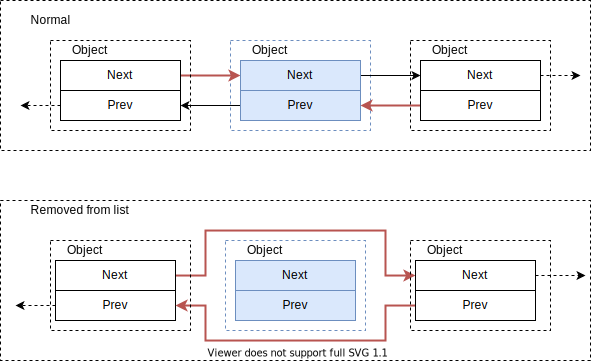
\includegraphics[scale=0.7]{images/dkom.png}
\end{figure}

The process list is a doubly-linked list, by removing the index to the desired
process malware can hide from windows API enumeration and list traversing.

The doubly-linked lists of loaded modules, namely \texttt{in load}, \texttt{in
memory}, \texttt{in initilization}, can all be edited to remove the module. A
naive malware will remove itself from the \texttt{in load} list, but a
comparison with the other two lists can reveal the hidden module. A better
hiding malware will try to remove itself from these three lists.

If the malware wants to hide one of its threads, it removes the thread from the
threads list, the pointer to the thread list is \texttt{ThreadListHead} in
\texttt{\_EPROCESS}.

Removing a node from the linked list is a common task, but DKOM is not limited
to these techniques, the malware can edit many members. An old
research\cite{robussignature} made by Brendan on Windows XP reveals that of the
72 selective members from selective structures, 29 members can be modified
without affecting, crashing, the system.  However, this research needs to be
updated with Windows 10. From the research results, malware can edit many
members, some of which will make them hidden from the system without breaking
the system.
